\begin{enumerate}
\item
\begin{align}
\begin{split}
\myvec{1 & 1 }\vec{x}&=5
\\
\myvec{2 & 2 }\vec{x}&=10
\end{split}
\end{align}
The above equations can be expressed as the matrix equation
\begin{align}
\myvec{1 & 1\\2 & 2} \vec{x} = \myvec{5\\10}
\end{align}
%
The augmented matrix for the above equation is row reduced as follows
\begin{align}
\myvec{1 & 1 & 5\\2 & 2 & 10} 
\xleftrightarrow {R_2\leftarrow R_2 -2R_1}\myvec{1 & \ 1 & 5 \\0 & 0 & 0 }
\end{align}
%
$\because$ row reduction of the $2\times 3$ matrix
%
\begin{align}
\myvec{1 & 1 & 5\\0 & 0 & 0} 
\end{align}
%
results in a matrix with 1 nonzero row, its rank is 1. 
%
Similarly, the rank of the matrix 
\begin{align}
\myvec{1 & 1 \\2 & 2 } 
\end{align}
%
is also 1.
%
\begin{align}
\because Rank \myvec{1 & 1\\2 & 2} &= Rank\myvec{1 & 1 & 5\\2 & 2 & 10} \nonumber\\
 &=dim \myvec{1 & 1\\2 & 2}\nonumber\\
 &=1
\end{align}
$\therefore$ the  lines in \eqref{linform/2/8/1.0.1} have infinitely many solutions and concide as seen in Fig. \ref{linform/2/8/fig:SAME LINES.}. The given lines are consistent.
%
\begin{figure}[ht!]
\centering
    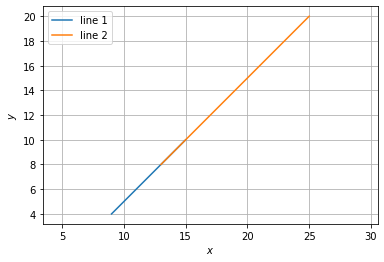
\includegraphics[width=\columnwidth]{solutions/su2021/2/8/ASSIGNMENT2/consistent.png}
    \caption{SAME LINES}
    \label{linform/2/8/fig:SAME LINES.}
\end{figure} 

\item
\begin{align}
\begin{split}
\myvec{1 & -1 }\vec{x}&=8  
\\
\myvec{3 & -3 }\vec{x}&=16
\end{split}
\end{align}
The above equations can be expressed as the matrix equation
\begin{align}
\myvec{1 & -1\\3 & -3}
\vec{x} = \myvec{8\\16}
\end{align}
%
The augmented matrix for the above equation is row reduced as follows
\begin{align}
\myvec{1 & -1 & 8\\3 &-3 & 16 }
\xleftrightarrow {R_2\leftarrow R_2-3R_1}\myvec{1 & -1 & 8 \\0 & 0 & -8}
\\
\end{align}
%
$\because$ row reduction of the $2\times 3$ matrix
%
\begin{align}
\myvec{1 & -1 & 8\\3 & -3 & 16}
\end{align}
%
results in a matrix with 2 nonzero rows, its rank is 2. 
%
Similarly, the rank of the matrix 
\begin{align}
\myvec{1 & -1 \\3 & -3 } 
\end{align}
%
is also 1.
%
\begin{align}
\because Rank \myvec{1 & -1\\3 & -3} \ne Rank\myvec{1 & -1 & 8\\3 & -3 & 16}\nonumber\\
\end{align}
$\therefore$ Given lines \eqref{linform/2/8/1.0.2} have no solution and are parallel as can be seen in Fig. \ref{linform/2/8/fig: PARALLEL lines.}
\begin{figure}[ht]
    \centering
   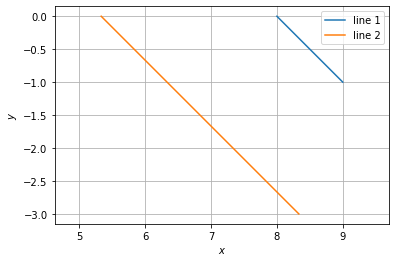
\includegraphics[width=\columnwidth]{solutions/su2021/2/8/ASSIGNMENT2/inconsistent.png}
    \caption{Parallel lines}
    \label{linform/2/8/fig: PARALLEL lines.}
\end{figure}    
